\section{Simulations}\label{sec:simulations}

In this chapter, we will test the previously described MPC in a virtual environment. Throughout the simulations, the whole complexity of the humanoid will be condensed in a single point, representing its CoM.\\
The objective of this set of tests is to prove that, using the inputs provided by the MPC proposed by Peng et al. in \cite{peng_main_paper} and developed by us, a robot is able to reach a user-defined goal, while avoiding collisions with all the obstacles in the environment.\\
The hyperparameters used in the following simulations are summarized in Table \ref{table:sim_params}.

\begin{table}[h]
        \begin{tabular}{ |p{4cm}||p{4cm}| }
             \hline
             \multicolumn{2}{|c|}{Simulation Parameters} \\
             \hline
             \textbf{Parameter} & \textbf{Value}\\
             \hline
             $\alpha$   & 3.6 \\
             CoM height & 1 \si{\meter} \\
             Step duration ($T$) & 0.4 \si{\second} \\
             $\left( l_{x_{\max}}, l_{y_{\max}} \right)$ & $\left( 0.1, 0.1 \right)  \;\si{\meter}$ \\
             $\left( l_{x_{\min}}, l_{y_{\min}} \right)$ & $\left( -0.1, -0.1 \right)  \;\si{\meter}$ \\
             $\left( v_{x_{min}},\, v_{y_{min}} \right)$ & $\left( -0.1,\, 0.1 \right)$ \si{\meter\per\second}\\
             $\left( v_{x_{max}},\, v_{y_{max}} \right)$ & $\left( 0.8,\, 0.4 \right)$ \si{\meter\per\second}\\
             \hline
        \end{tabular}
    \centering
    \caption{The MPC and LIP parameters used for all the simulations in this chapter.}
    \label{table:sim_params}
\end{table}

\subsection{Simple Environment}\label{subsec:sim_simple_env}
The first simulation takes place in a basic environment: the humanoid is positioned at $(0,\,3)$ with orientation $\theta = 0$, and the goal position is $(6,\,-3)$. In between, we placed 3 obstacles with a quasi-circular shape. The choice of approximating circles with polygons was made to comply with the CBF computation described in \ref{subsec:ldcbf}. The results are shown in Figures \ref{fig:sim1_evol} and \ref{fig:sim1_frames}.

By inspecting the plots, we see that, at the beginning of the simulation, a high turning velocity $\omega$ is commanded in order to make the robot point toward the goal. In the meantime, the MPC provides new footstep positions but, due to the maneuverability constraint, the high turning rate limits the velocity along the sagittal axis. This is the reason why the first peak in the longitudinal velocities plot is lower than the subsequent ones.\\
At this point, the robot moves forward to the goal and the orientation is kept constant. Nevertheless, there are some oscillations in the plot of the local velocities. This is a regular behavior. The chattering of the longitudinal velocities is due to the fact that the humanoid makes a larger step followed by a smaller one, to preserve equilibrium. The velocity along the lateral axis oscillates becuase, at the end of each step, the humanoid changes the stance foot by \textit{falling} on the opposite side, and it results in the lateral velocity changing sign. This behavior is less evident while turning.\\
Around the second 10 of the simulation (4th frame of Figure \ref{fig:sim1_frames}), the humanoid approaches one of the obstacles. It is unable to go forward, as this would lead the CoM into the circle. To keep the robot in the safe area defined by the LDCBF, the new MPC solution makes the humanoid move laterally. Thus, it can successfully avoid the obstacle. In this case, \textit{side walking} occurs because the precomputed value of $\omega$ only aims at aligning the sagittal axis of the robot with the goal, and, once it is achieved, the turning rate is kept constant. Consequently, the humanoid can only escape the obstacle while facing the goal. This movement explains the noticable variations in the lateral velocity plots between seconds 10 and 13.\\
The humanoid can, then, realign itself (producing a minimal alteration in the $\theta$ and $\omega$ plots) and continue navigating to the goal, which it ultimately reaches successfully.\\
The humanoid's Zero Moment Point (ZMP) is evaluated only at the end of each step, when it is coincident with the stance foot position. In the CoM-ZMP plot we observe the typical behavior, where the ZMP is constantly oscillating around the CoM (according to the LIP dynamics), while staying in the support polygon. However, a variation occurs during the side-waling phase, where the ZMP pushes the CoM laterally in order to avoid the obstacle.

\begin{figure}[H]
    \centering
    \begin{subfigure}{0.45\linewidth}
        \centering
        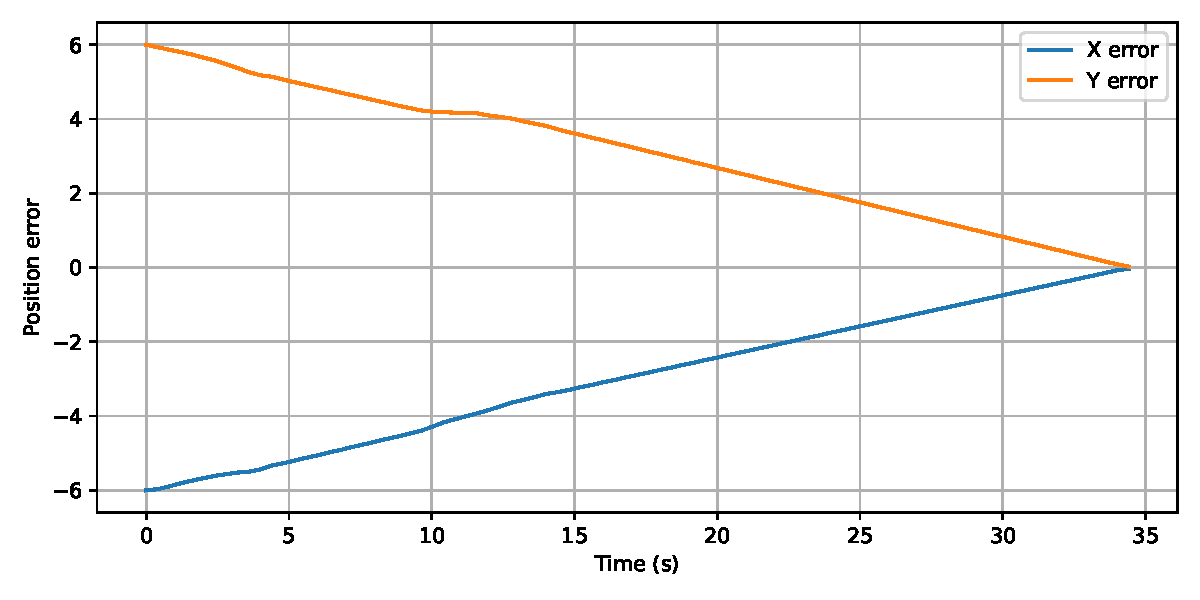
\includegraphics[width=\linewidth]{figures/Simulations/sim1circles/evolution_0.pdf}
    \end{subfigure}
    \begin{subfigure}{0.45\linewidth}
        \centering
        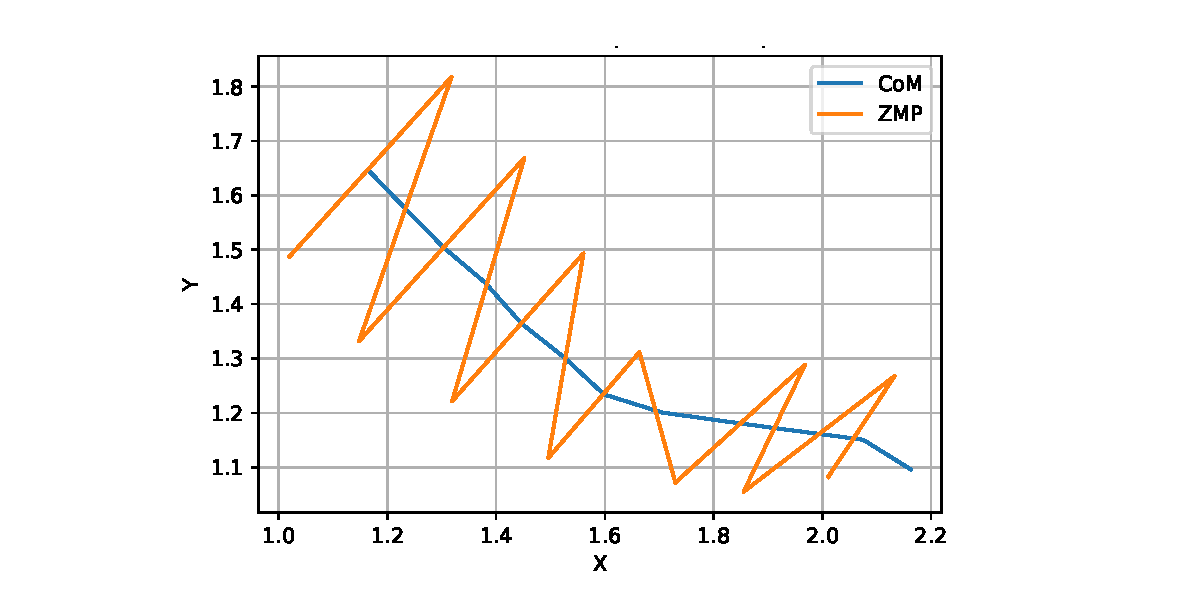
\includegraphics[width=\linewidth]{figures/Simulations/sim1circles/evolution_5.pdf}
    \end{subfigure}
    \hfill
    \begin{subfigure}{0.45\linewidth}
        \centering
        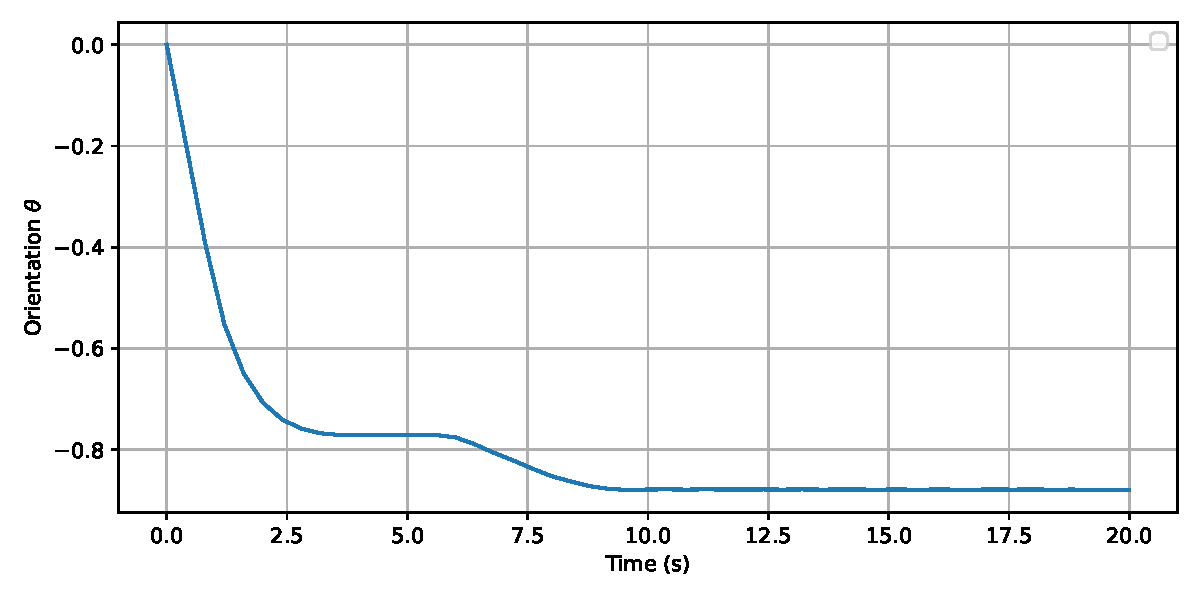
\includegraphics[width=\linewidth]{figures/Simulations/sim1circles/evolution_2.pdf}
    \end{subfigure}
    \begin{subfigure}{0.45\linewidth}
        \centering
        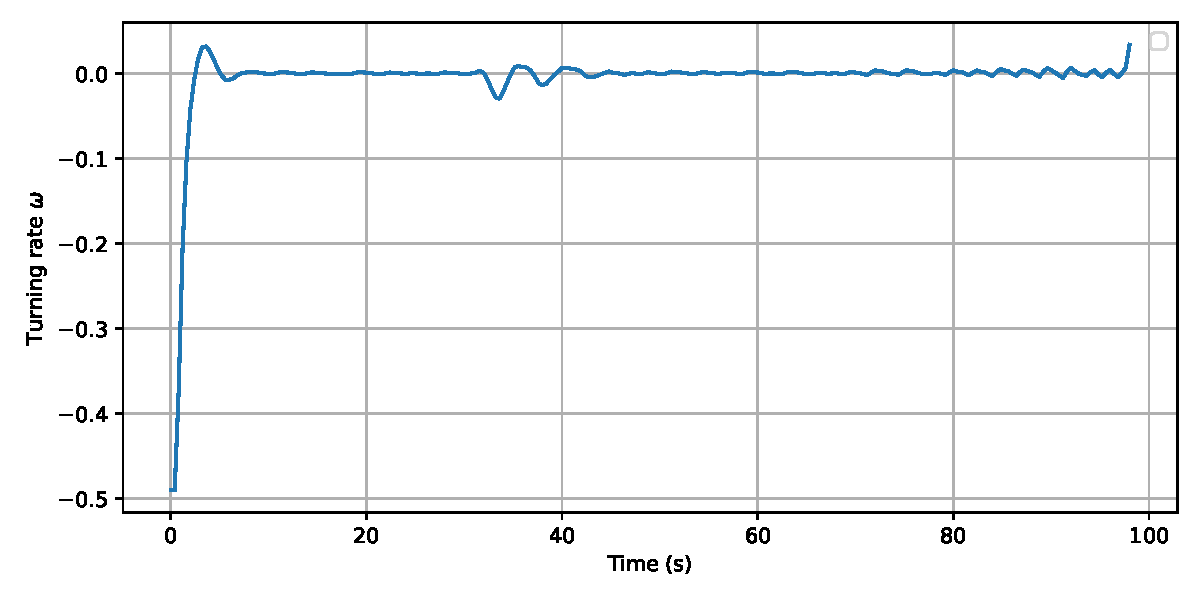
\includegraphics[width=\linewidth]{figures/Simulations/sim1circles/evolution_3.pdf}
    \end{subfigure}
    \hfill
    \begin{subfigure}{0.45\linewidth}
        \centering
        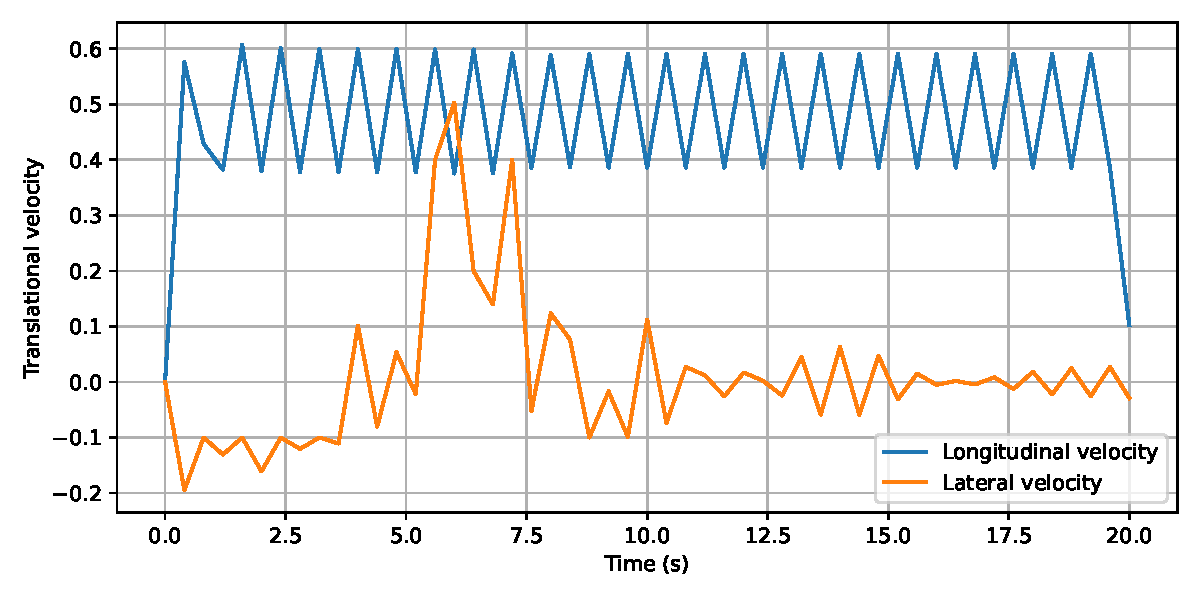
\includegraphics[width=\linewidth]{figures/Simulations/sim1circles/evolution_1.pdf}
    \end{subfigure}
    \caption{These figures depict the evolution of the humanoid's state and the input throughout the simulation in the base environment employing our LDCBF. The top-left plot shows the error between the CoM and the goal position, while the top-right represents the trajectory of the ZMP and the CoM in the Cartesian plane. The middle left and right plots show the theta and omega evolution, respectively. The bottom plot shows the CoM longitudinal and lateral velocities.}
    \label{fig:sim1_evol}
\end{figure}

\newpage
\begin{figure}[H]
    \centering
    % First row
    \begin{subfigure}{0.35\textwidth}
        \centering
        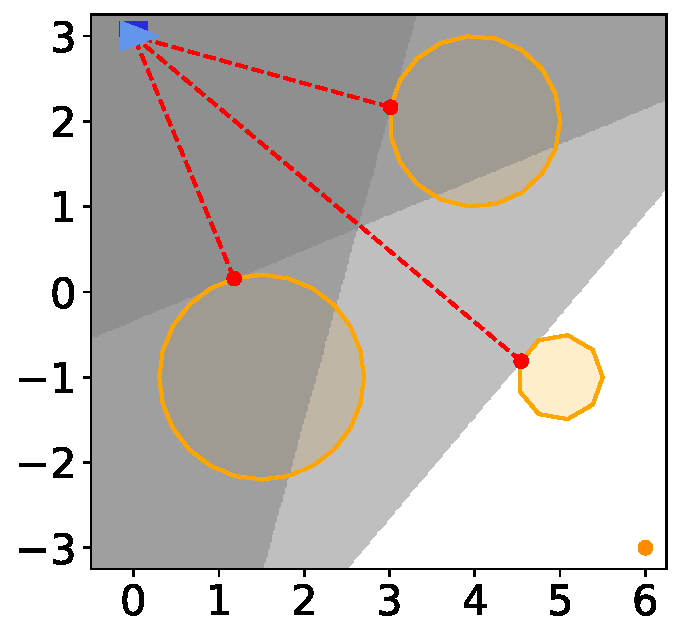
\includegraphics[width=\textwidth]{figures/Simulations/sim1circles/frame_0.pdf}
    \end{subfigure}%
    \hfil
    \begin{subfigure}{0.35\textwidth}
        \centering
        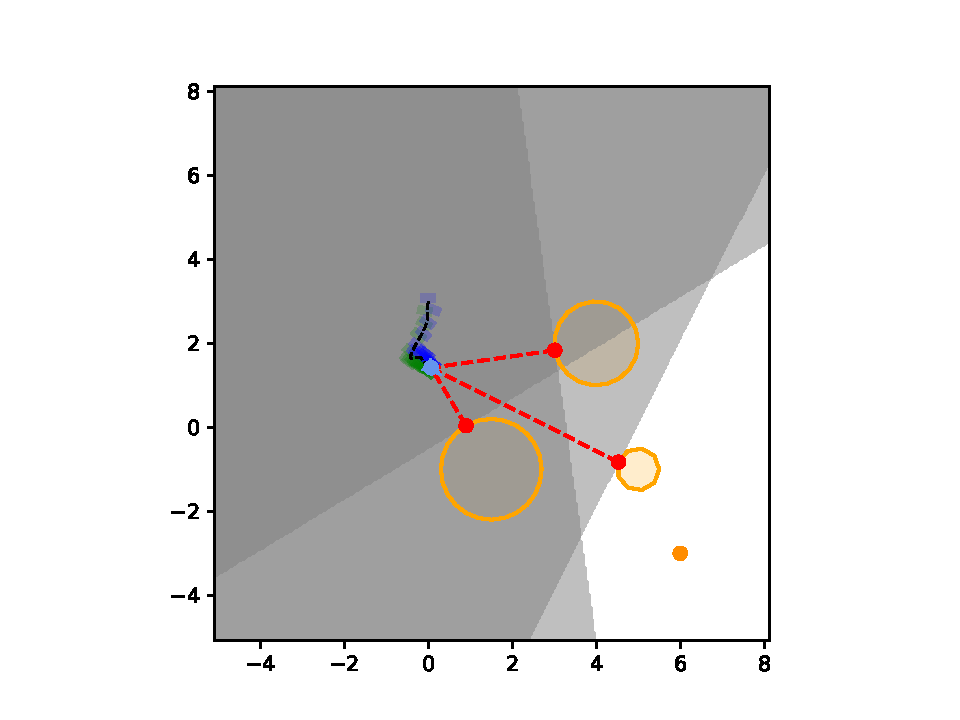
\includegraphics[width=\textwidth]{figures/Simulations/sim1circles/frame_1.pdf}
    \end{subfigure}%
    
    \begin{subfigure}{0.35\textwidth}
        \centering
        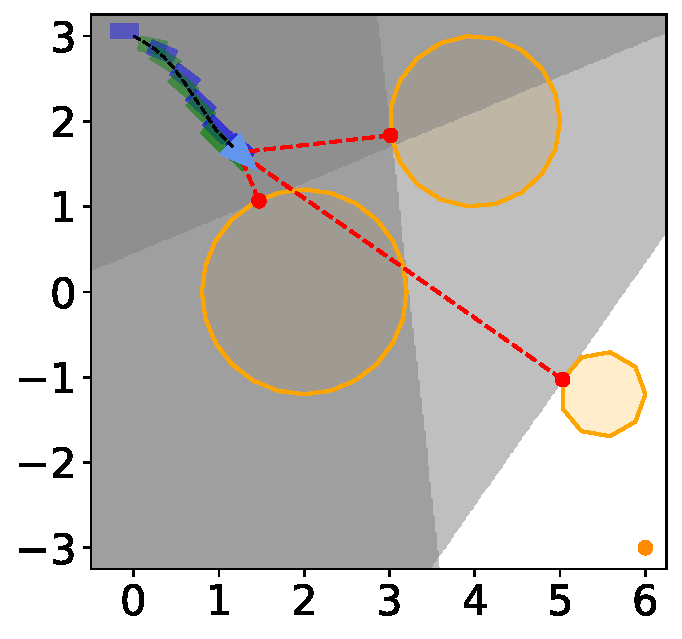
\includegraphics[width=\textwidth]{figures/Simulations/sim1circles/frame_2.pdf}
    \end{subfigure}%
    \hfil
    \begin{subfigure}{0.35\textwidth}
        \centering
        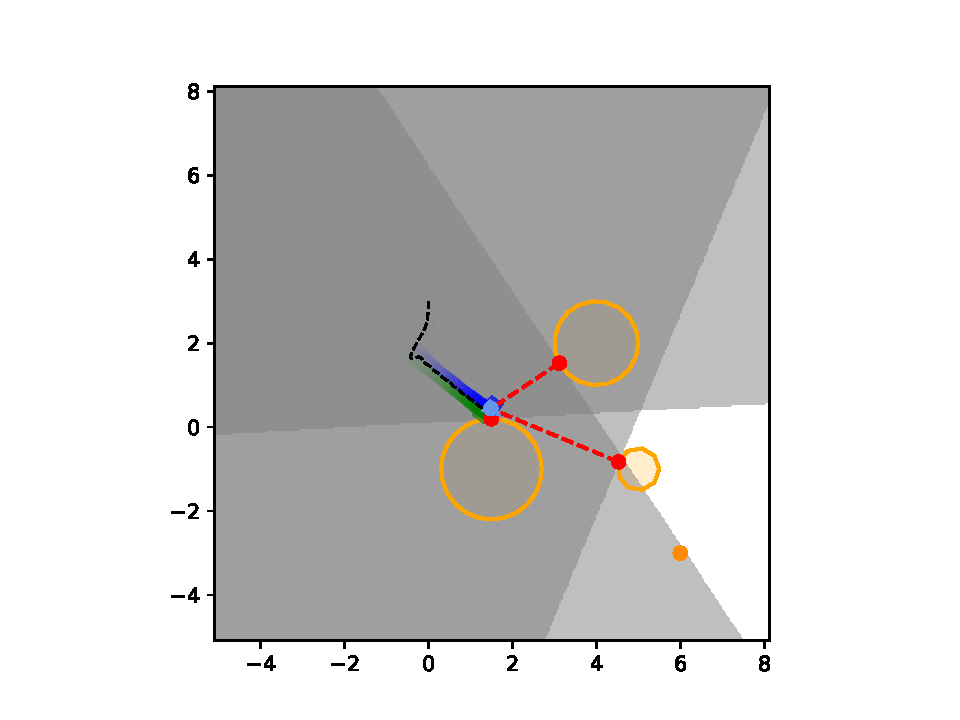
\includegraphics[width=\textwidth]{figures/Simulations/sim1circles/frame_3.pdf}
    \end{subfigure}%

    \begin{subfigure}{0.35\textwidth}
        \centering
        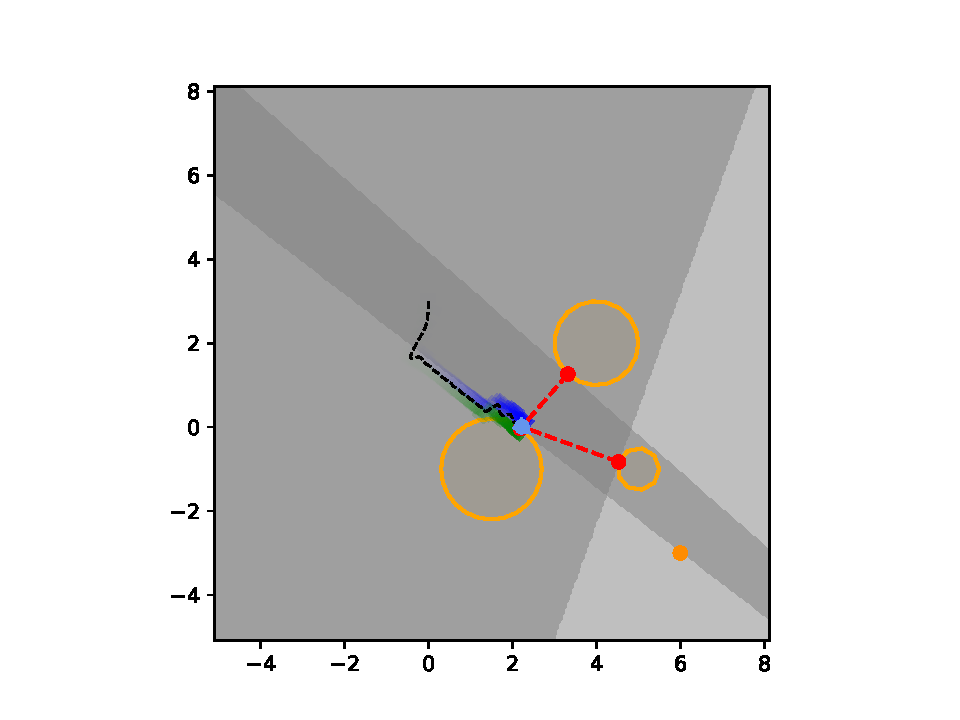
\includegraphics[width=\textwidth]{figures/Simulations/sim1circles/frame_4.pdf}
    \end{subfigure}
    \hfil
    \begin{subfigure}{0.35\textwidth}
        \centering
        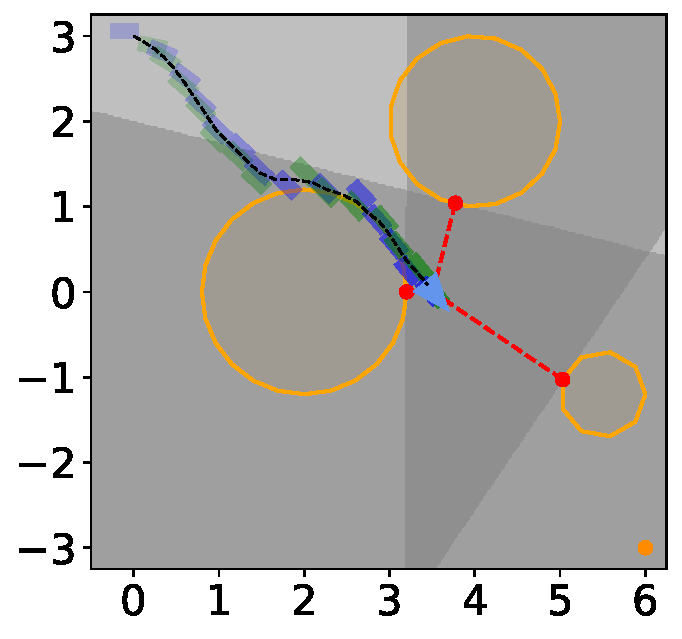
\includegraphics[width=\textwidth]{figures/Simulations/sim1circles/frame_5.pdf}
    \end{subfigure}%

    \begin{subfigure}{0.35\textwidth}
        \centering
        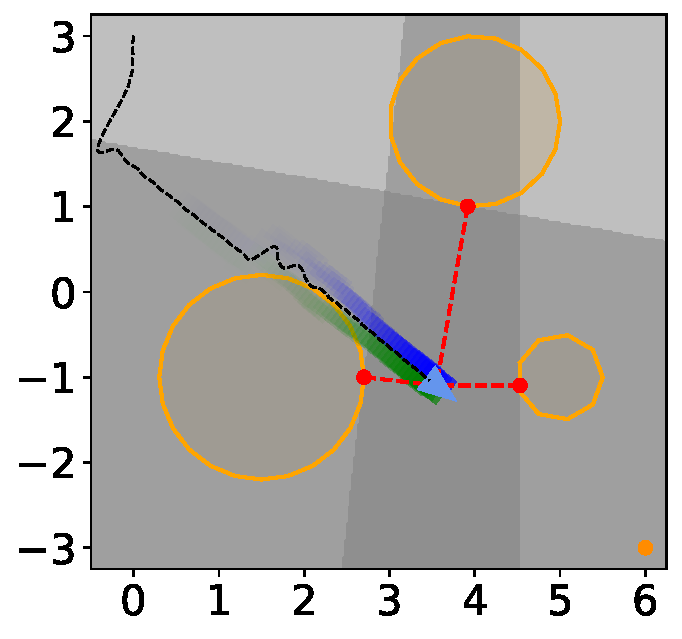
\includegraphics[width=\textwidth]{figures/Simulations/sim1circles/frame_6.pdf}
    \end{subfigure}%
    \hfil
    \begin{subfigure}{0.35\textwidth}
        \centering
        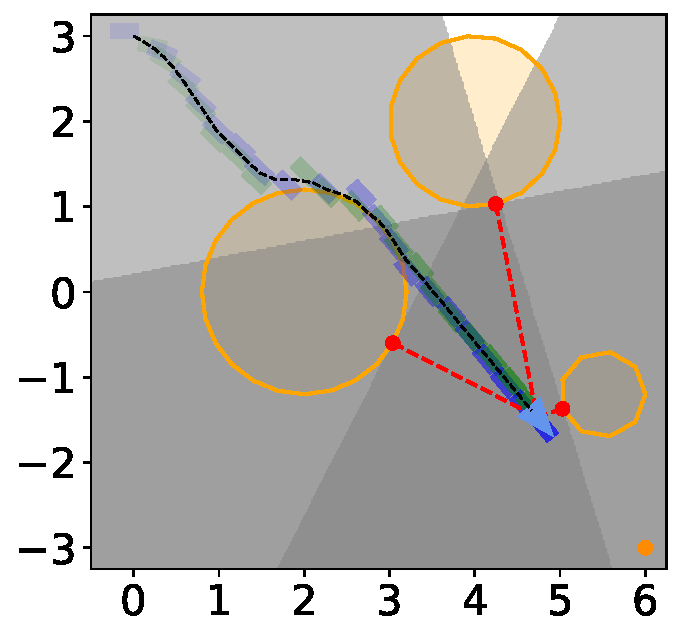
\includegraphics[width=\textwidth]{figures/Simulations/sim1circles/frame_7.pdf}
    \end{subfigure}%

    \begin{subfigure}{0.35\textwidth}
        \centering
        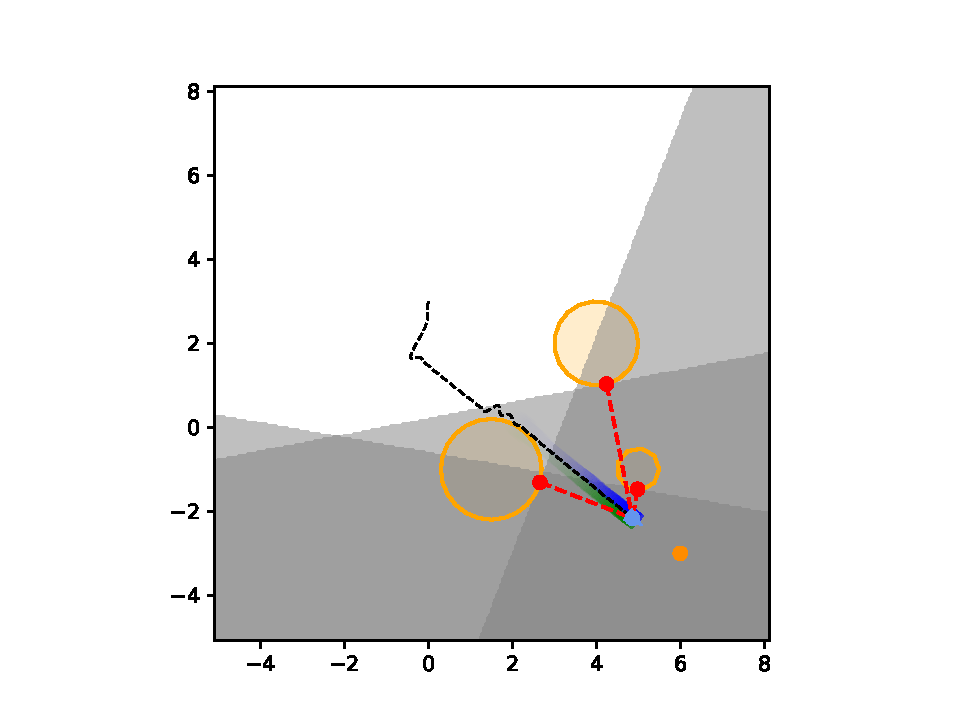
\includegraphics[width=\textwidth]{figures/Simulations/sim1circles/frame_8.pdf}
    \end{subfigure}%
    \hfil
    \begin{subfigure}{0.35\textwidth}
        \centering
        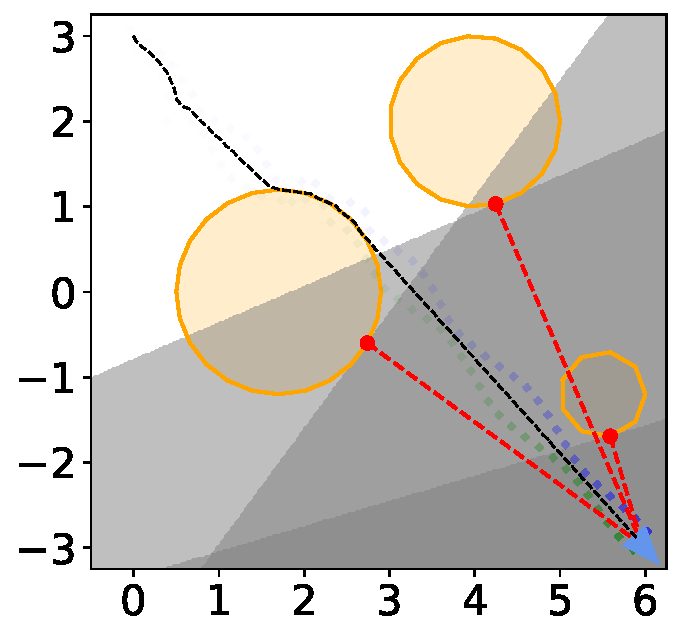
\includegraphics[width=\textwidth]{figures/Simulations/sim1circles/frame_9.pdf}
    \end{subfigure}
    \caption[short]{Simulation with circular obstacles.}
    %\caption[short]{This sequence of frames illustrates the robot's trajectory to the goal. Obstacles are represented with orange shapes. The humanoid is represented by an isosceles triangle whose sagittal axis is aligned with the robot's. Green rectangles mark right footsteps, while blue rectangles mark left ones. Each frame shows the vectors $\eta$ and $c$ along with the safe area associated with each obstacle. The darkest region represents the intersection of these semi-planes, which is the overall safe area.}
    \label{fig:sim1_frames}
\end{figure}
\thispagestyle{empty}

\subsubsection{Simulation employing our LDCBF}
From an accurate analysis of the previous simulation's frames, it can be observed that, despite the robot accomplishing the mission of reaching the goal while satisfying all the constraints, when it gets very close to the obstacles, its feet overlap with the obstacles. This occurs due to the LDCBF defined by Peng et al., which only ensures that the CoM never collides with the obstacles. However, this strategy produces a path that is impractical for the full-body motion of the humanoid (as already pointed out in \ref{subsec:ldcbf_variant}). Therefore, we proposed our variant of their LDCBF, and in Figures \ref{fig:sim1_delta_evol} and \ref{fig:sim1_delta_frames} we show the results of the simulation that constraints the MPC with the LDCBF defined at (\ref{eq:ldcbf_variant}), setting $\delta=0.3$.

From the plots, we notice that the robot reaches the boundary of the safe area -- no longer coincident with the obstacle's edge -- earlier than the previous simulation, and the longitudinal velocity is drastically reduced to stay inside the boundary. Then, it reorients itself with the modality exposed before. The same situation arises around the second 27 of the simulation, when the robot moves from its trajectory to keep a distance $\delta$ from the last obstacle.

The simulation frames in Figure \ref{fig:sim1_delta_frames} reveal that the humanoid's footsteps never intersect the obstacles. Subsequently, the LDCBF contributed to designing a motion plan suitable for the humanoid in real-world conditions.

\begin{figure}[H]
    \centering
    \begin{subfigure}{0.45\linewidth}
        \centering
        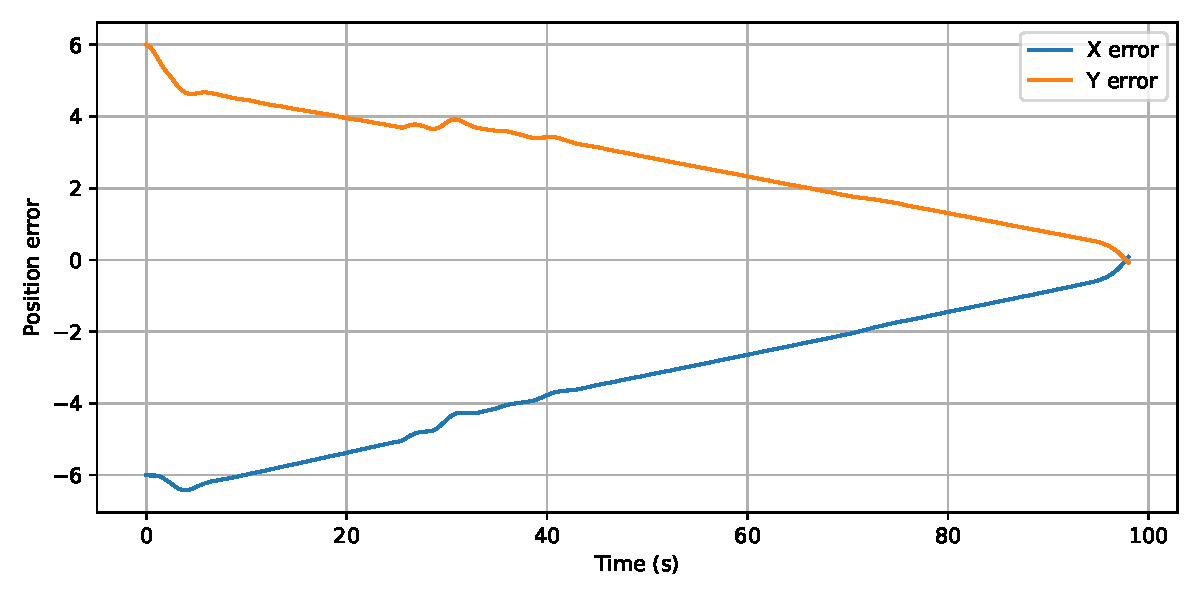
\includegraphics[width=\linewidth]{figures/Simulations/sim1circles_delta/evolution_0.pdf}
    \end{subfigure}
    \begin{subfigure}{0.45\linewidth}
        \centering
        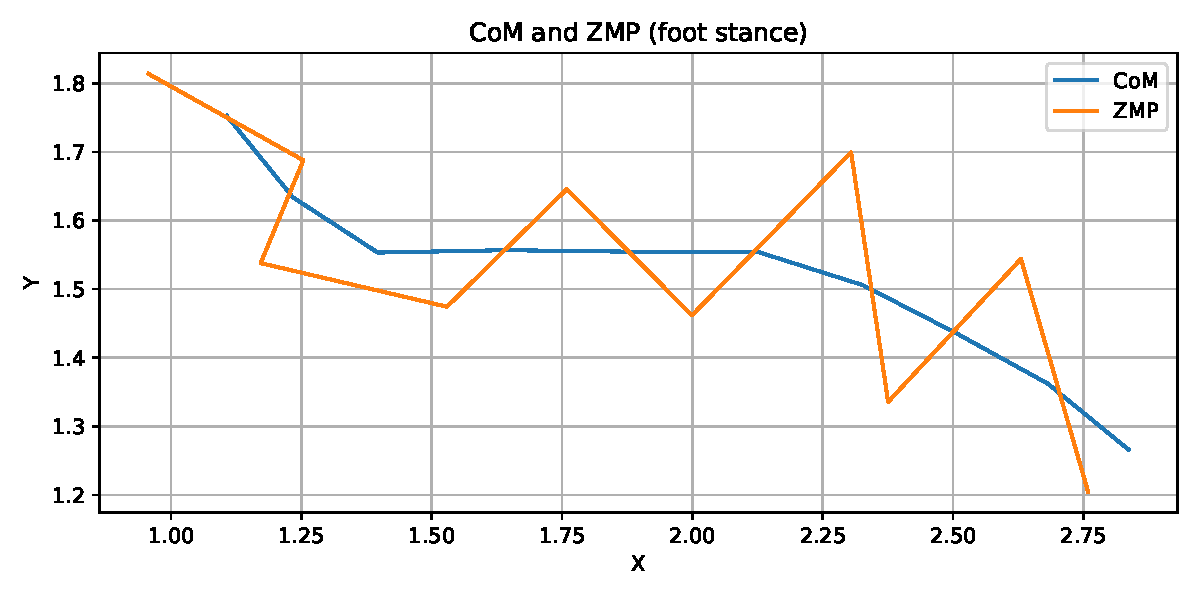
\includegraphics[width=\linewidth]{figures/Simulations/sim1circles_delta/evolution_5.pdf}
    \end{subfigure}
    \hfill
    \begin{subfigure}{0.45\linewidth}
        \centering
        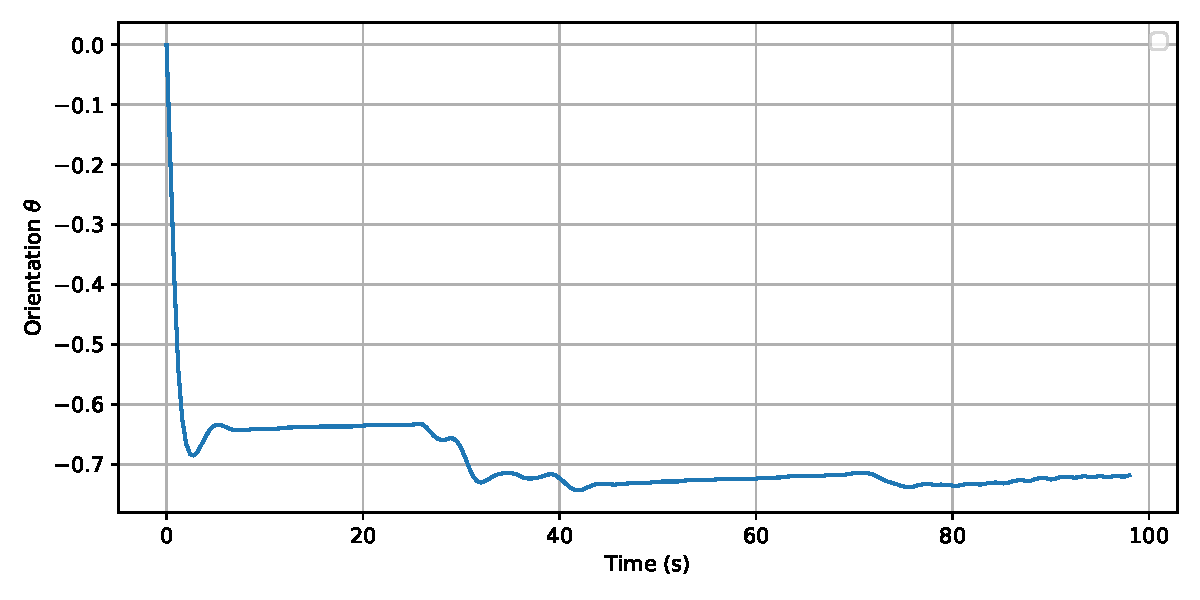
\includegraphics[width=\linewidth]{figures/Simulations/sim1circles_delta/evolution_2.pdf}
    \end{subfigure}
    \begin{subfigure}{0.45\linewidth}
        \centering
        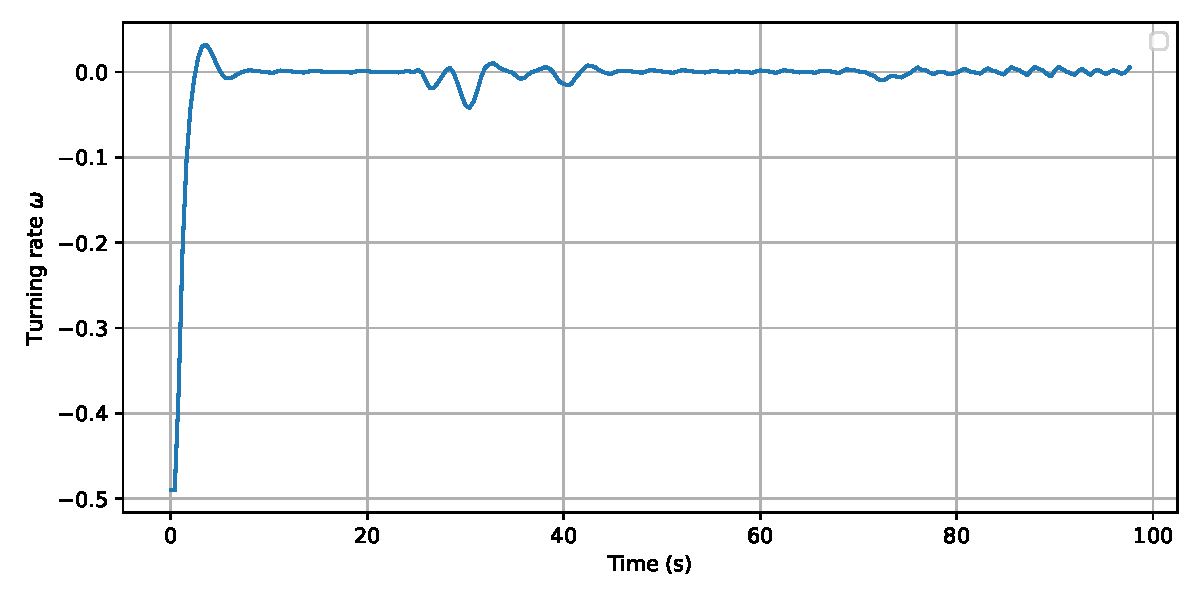
\includegraphics[width=\linewidth]{figures/Simulations/sim1circles_delta/evolution_3.pdf}
    \end{subfigure}
    \hfill
    \begin{subfigure}{0.45\linewidth}
        \centering
        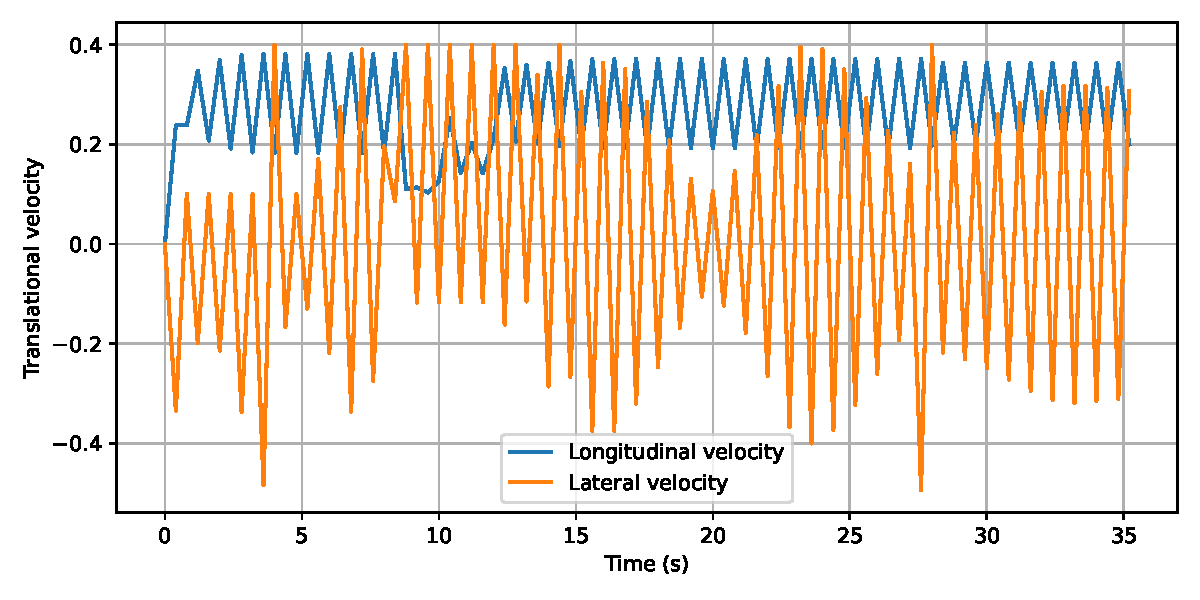
\includegraphics[width=\linewidth]{figures/Simulations/sim1circles_delta/evolution_1.pdf}
    \end{subfigure}
    \caption{These figures depict the evolution of the humanoid's state and the input throughout the simulation in the base environment employing our LDCBF.}
    \label{fig:sim1_delta_evol}
\end{figure}

\newpage
\begin{figure}[H]
    \centering
    % First row
    \begin{subfigure}{0.35\textwidth}
        \centering
        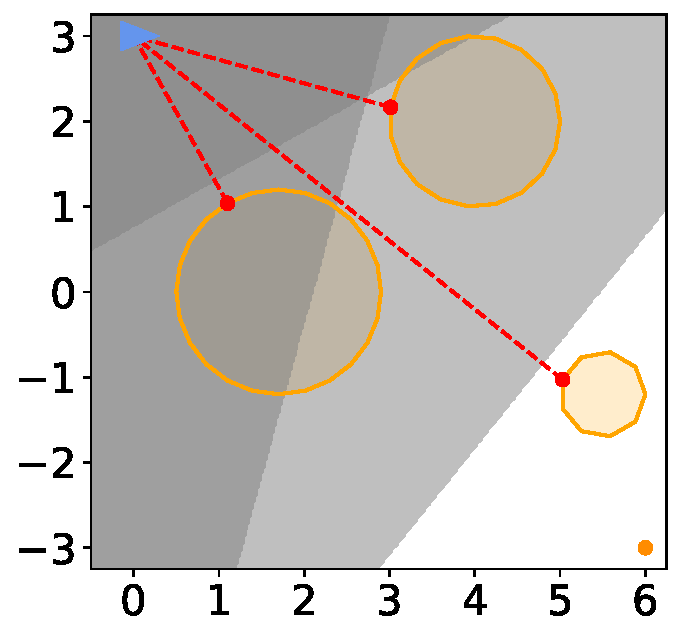
\includegraphics[width=\textwidth]{figures/Simulations/sim1circles_delta/frame_0.pdf}
    \end{subfigure}%
    \hfil
    \begin{subfigure}{0.35\textwidth}
        \centering
        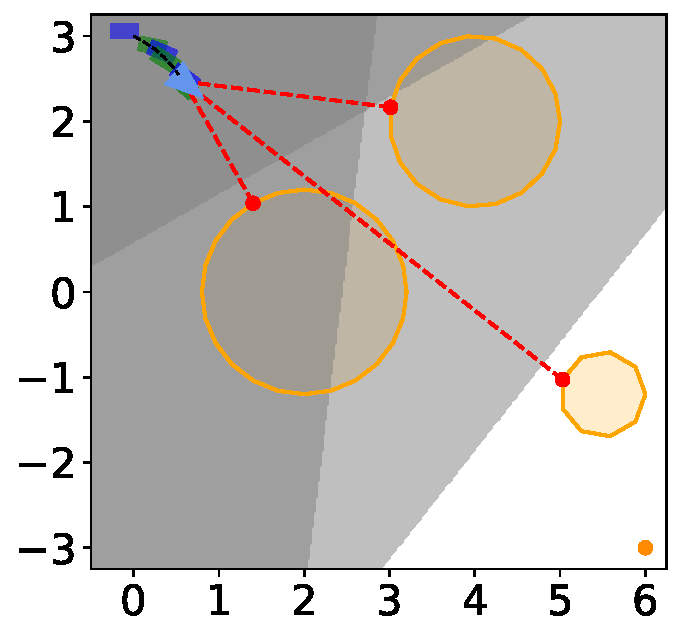
\includegraphics[width=\textwidth]{figures/Simulations/sim1circles_delta/frame_1.pdf}
    \end{subfigure}%

    \begin{subfigure}{0.35\textwidth}
        \centering
        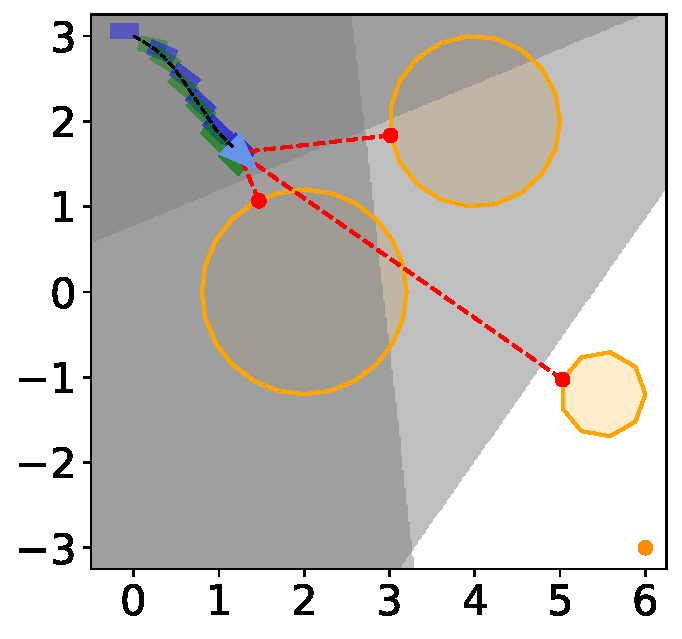
\includegraphics[width=\textwidth]{figures/Simulations/sim1circles_delta/frame_2.pdf}
    \end{subfigure}%
    \hfil
    \begin{subfigure}{0.35\textwidth}
        \centering
        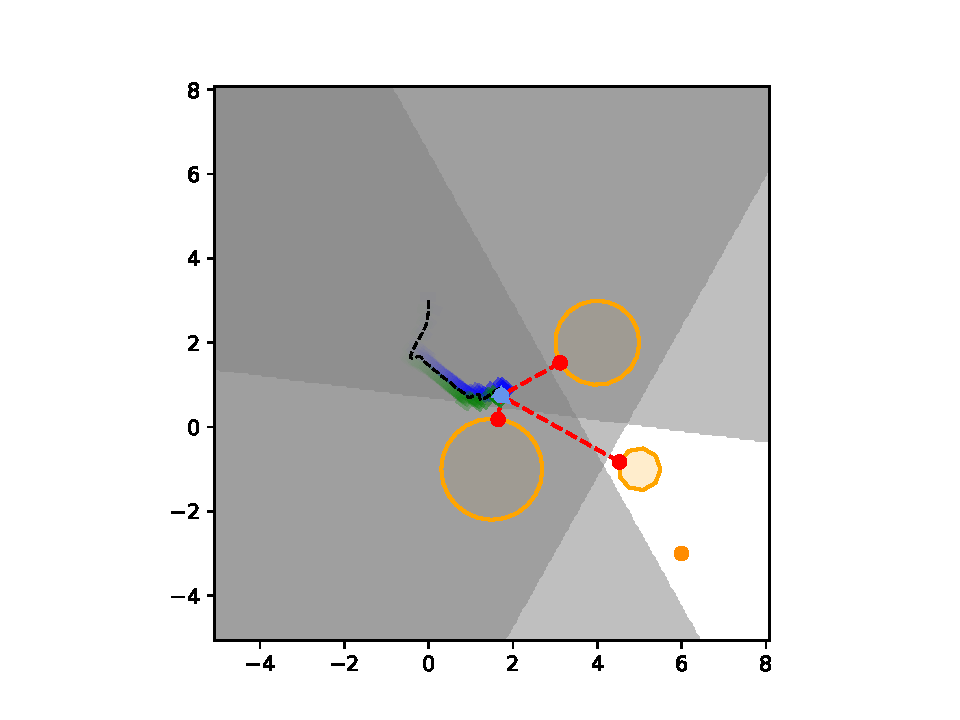
\includegraphics[width=\textwidth]{figures/Simulations/sim1circles_delta/frame_3.pdf}
    \end{subfigure}%
    
    \begin{subfigure}{0.35\textwidth}
        \centering
        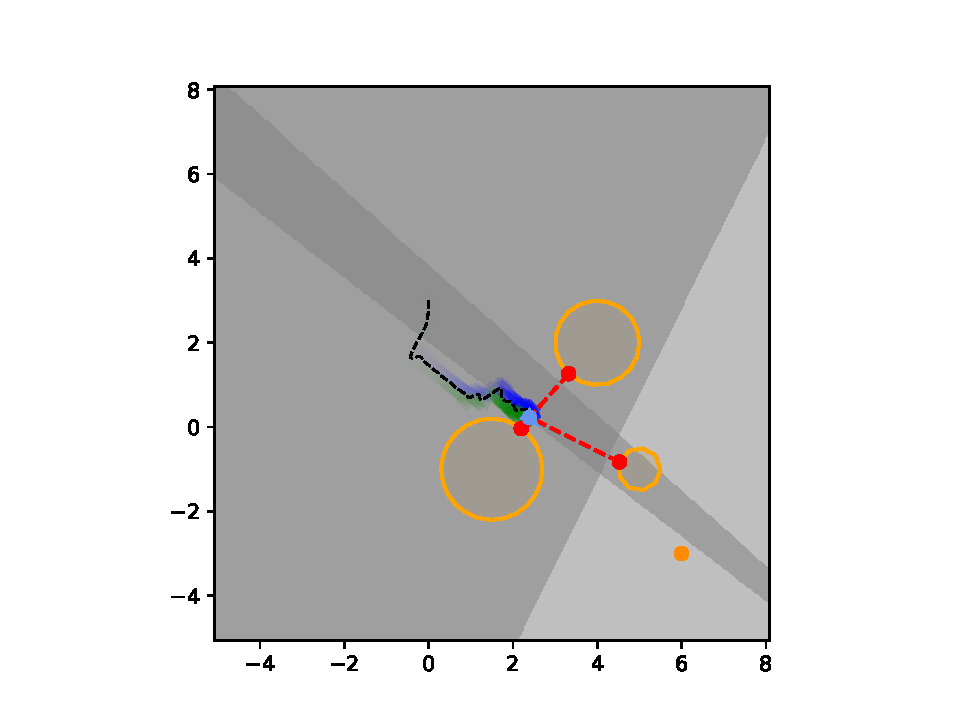
\includegraphics[width=\textwidth]{figures/Simulations/sim1circles_delta/frame_4.pdf}
    \end{subfigure}
    \hfil
    \begin{subfigure}{0.35\textwidth}
        \centering
        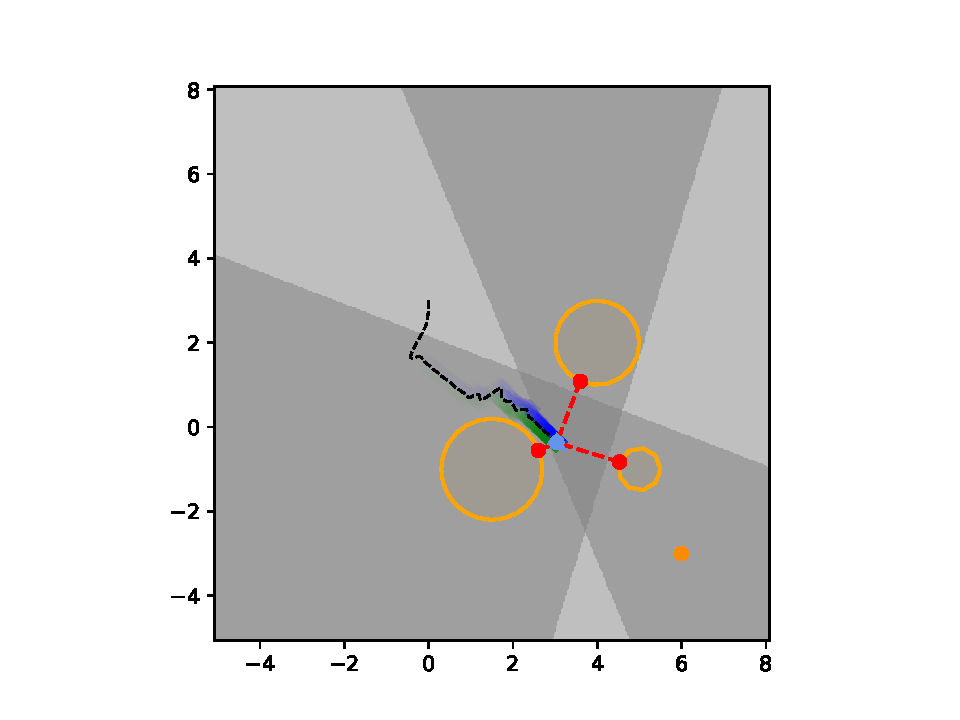
\includegraphics[width=\textwidth]{figures/Simulations/sim1circles_delta/frame_5.pdf}
    \end{subfigure}%
    
    \begin{subfigure}{0.35\textwidth}
        \centering
        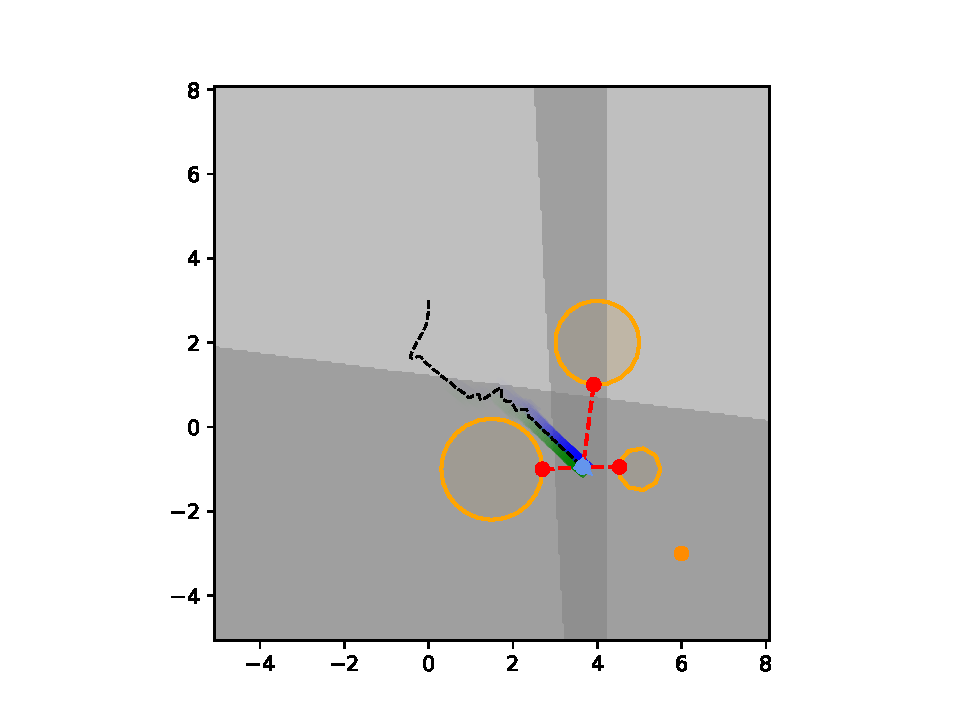
\includegraphics[width=\textwidth]{figures/Simulations/sim1circles_delta/frame_6.pdf}
    \end{subfigure}%
    \hfil
    \begin{subfigure}{0.35\textwidth}
        \centering
        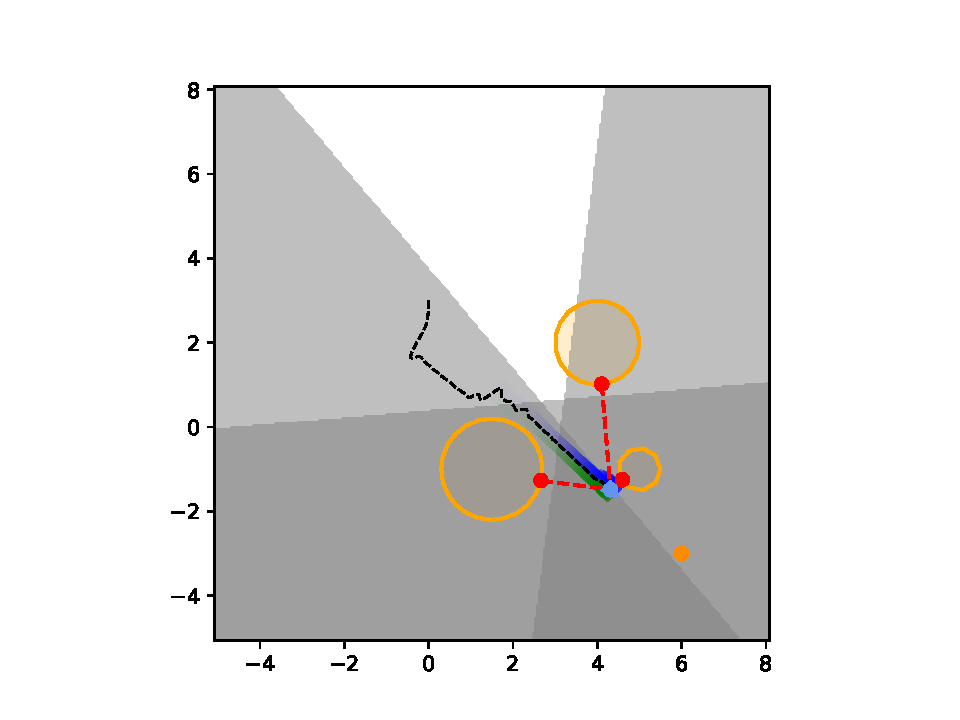
\includegraphics[width=\textwidth]{figures/Simulations/sim1circles_delta/frame_7.pdf}
    \end{subfigure}%

    \begin{subfigure}{0.35\textwidth}
        \centering
        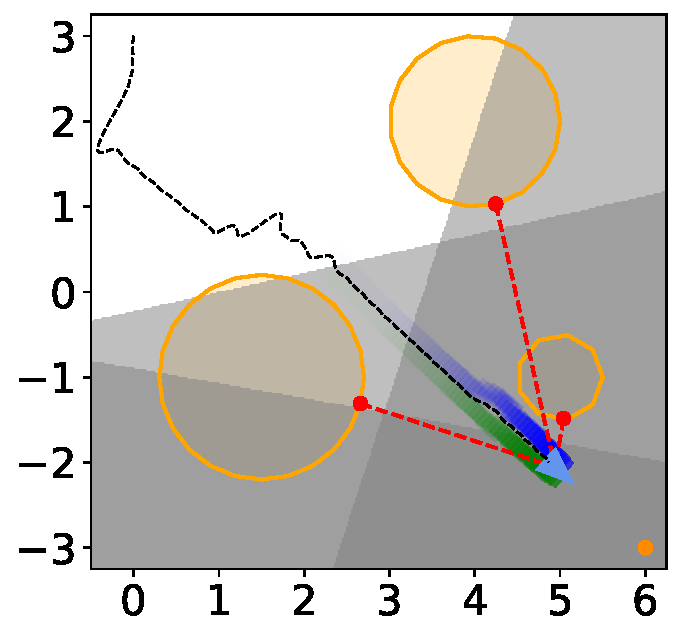
\includegraphics[width=\textwidth]{figures/Simulations/sim1circles_delta/frame_8.pdf}
    \end{subfigure}%
    \hfil
    \begin{subfigure}{0.35\textwidth}
        \centering
        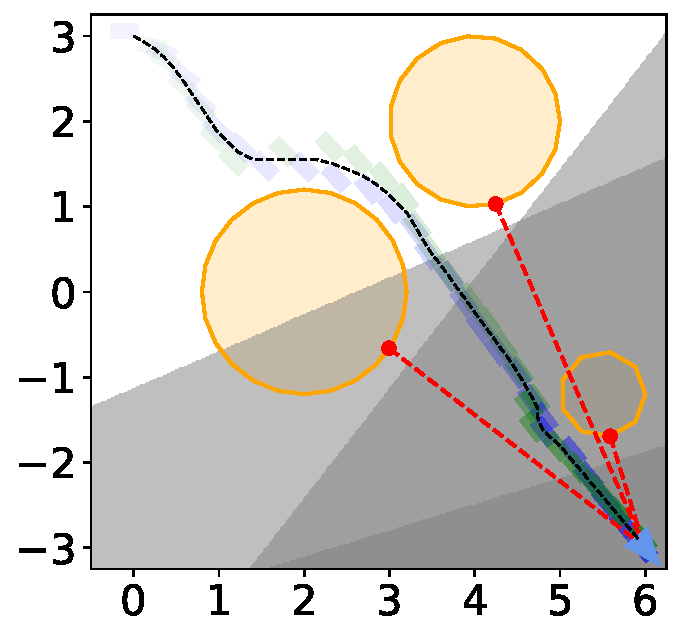
\includegraphics[width=\textwidth]{figures/Simulations/sim1circles_delta/frame_9.pdf}
    \end{subfigure}
    
    \caption[short]{Simulation with circular obstacles employing our LDCBF (with $\delta$ = 0.3).}
    %\caption[short]{This sequence of frames illustrates the robot's trajectory to the goal for the simulation in the base environment employing our LDCBF. With this modification, the darkest region (i.e., the overall safe area) never touches the obstacles boundaries, but is always at a user-defined distance $\delta$.}
    \label{fig:sim1_delta_frames}
\end{figure}
\thispagestyle{empty}